\section{Multi-name models of default}
We consider credit derivatives whose underlying is a set of names (reference entities). A multi-name contract is associated with multiple credit events which trigger remedial payment to the protection buyer. The collateralized debt obligation (CDO) is one of the most popular multi-name credit derivatives. We want to look at the default correlation.

\subsection{A structual approach}
To model the default correlation consider the Black-Scholes-Merton (BSM) structural model of default with default defined as

$$
\tau= \begin{cases}T, & \text { if } V_{T}<F \\ \infty & \text { if } V_{T} \geq F\end{cases}
$$

where $F$ is the face value of the debt and $V_{T}$ is the asset values at maturity. Hence, it is the asset values $V_{T}$ at maturity $T$ that is the quantity of interest. Assuming $T=1$ and defining the return on the asset values $\tilde{R}$ over the period from 0 to $T$ as

$$
\e^{\tilde{R}}=\frac{V_{1}}{V_{0}}=\frac{V_{0} \e^{\left(\mu-\frac{\sigma^{2}}{2}\right)}}{V_{0}}
$$

where the last equality holds since $V_{T}$ is log-normally distributed in the BSM model. Taking the logarithm on both sides we have

$$
\tilde{R} \sim N\left(\mu-\frac{\sigma^{2}}{2}, \sigma^{2}\right)
$$

Likewise, the default can be written in terms of the return on the asset value

$$
\begin{gathered}
V_{1}<F, \\
\widehat{\Downarrow} \\
\tilde{R}=\ln \left(\frac{V_{1}}{V_{0}}\right)<\ln \left(\frac{F}{V_{0}}\right), \\
\widehat{\Downarrow} \\
R=\frac{\tilde{R}-\left(\mu-\frac{\sigma^{2}}{2}\right)}{\sigma}<\frac{\ln \left(\frac{F}{V_{0}}\right)-\left(\mu-\frac{\sigma^{2}}{2}\right)}{\sigma}=C,
\end{gathered}
$$

where $R$ is the standardized return on the firm value and the right hand side is a constant $C$. Thus, default of the firm can be written as

$$
R<C
$$

where $R$ is standard normally distributed.

\section{Introducing several companies}
We define the default of company $i$ as when the standardized return on owning the firm falls below a firm specific threshold $C_{i}$ at some future time $T$

$$
\text { Company } i \text { defaults at time } T \Longleftrightarrow R_{i} \leq C_{i}, \quad R_{i}=\frac{\tilde{R}_{i}-\E\left[\tilde{R}_{i}\right]}{\sqrt{\mathbb{V}\left[\tilde{R}_{i}\right]}}
$$

The standardization means all $R_{i}$ s in the portfolio have zero mean and unit variance. We assume that individual period returns $R_{i}$ are normally distributed. Thus, the default probabilities are

$$
q_{i}=\Q\left[R_{i} \leq C_{i}\right]=\Phi\left(C_{i}\right) \quad \Longrightarrow \quad C_{i}=\Phi^{-1}\left(q_{i}\right)
$$

with $\Phi(\cdot)$ the CDF of the standard normal distribution. Furthermore, assume that all returns are correlated through one common factor $\alpha$ by

$$
R_{i}=\beta_{i} \alpha+\sqrt{1-\beta_{i}^{2}} \epsilon_{i}
$$

where $\alpha$ and $\epsilon_{i}$ are independent and standard normally distributed. Also, the $\epsilon_{i}$ s are independent. (The common factor $\alpha$ could be interpreted as the standardized return on the stock market or the general state of the economy).

How are company returns correlated in this setting?

$$
\begin{aligned}
\operatorname{Cov}\left(R_{i}, R_{j}\right) & =\E\left[\left(R_{i}-\E\left[R_{i}\right]\right)\left(R_{j}-\E\left[R_{j}\right]\right)\right] \\
& =\E\left[R_{i} R_{j}\right] \\
& =\E\left[\beta_{i} \beta_{j} \alpha^{2}\right] \\
& =\beta_{i} \beta_{j} \\
& =\operatorname{corr}\left(R_{i}, R_{j}\right),
\end{aligned}
$$

since all the other random variables involved are independent and we have unit variance. Key advantage: Given a common factor $\alpha$ the returns are independent, observed by

$$
\begin{aligned}
& \E\left[R_{i} \mid \alpha\right]=\beta_{i} \alpha \\
& \mathbb{V}\left[R_{i} \mid \alpha\right]=\E\left[\left(R_{i}-\beta_{i} \alpha\right)^{2} \mid \alpha\right]=\E\left[\left(1-\beta_{i}^{2}\right) \epsilon_{i}^{2} \mid \alpha\right]=1-\beta_{i}^{2}
\end{aligned}
$$

Now, we can find the correlation of the returns given knowledge of the common factor $\alpha$

$$
\operatorname{Cov}\left(R_{i}, R_{j} \mid \alpha\right)=\sqrt{1-\beta_{i}^{2}} \sqrt{1-\beta_{j}^{2}} \E\left[\epsilon_{i} \epsilon_{j} \mid \alpha\right]=0
$$

since individual factors were assumed independent. From this, the convenient form of the default probability given $\alpha$ arises

$$
\begin{aligned}
q_{i}(\alpha) & =\Q\left[R_{i} \leq C_{i} \mid \alpha\right] \\
& =\Q\left[\left.\epsilon_{i} \leq \frac{C_{i}-\beta_{i} \alpha}{\sqrt{1-\beta_{i}^{2}}} \right\rvert\, \alpha\right] \\
& =\Phi\left(\frac{C_{i}-\beta_{i} \alpha}{\sqrt{1-\beta_{i}^{2}}}\right) \\
& =\Phi\left(\frac{\Phi^{-1}\left(q_{i}\right)-\beta_{i} \alpha}{\sqrt{1-\beta_{i}^{2}}}\right)
\end{aligned}
$$

which depends on $\beta_{i}$.

What are the correlation of defaults $\rho_{i, j}$ ? It has the form form

$$
\rho_{i, j}=\frac{q_{i \& j}-q_{i} q_{j}}{\sqrt{q_{i}\left(1-q_{i}\right)} \sqrt{q_{j}\left(1-q_{j}\right)}}=\frac{\Phi_{2}\left(C_{i}, C_{j} ; \beta_{i} \beta_{j}\right)-\Phi\left(C_{i}\right) \Phi\left(C_{j}\right)}{\sqrt{\Phi\left(C_{i}\right)\left(1-\Phi\left(C_{i}\right)\right)} \sqrt{\Phi\left(C_{j}\right)\left(1-\Phi\left(C_{j}\right)\right)}},
$$

using $q_{i}(\alpha)=\Phi\left(C_{i}\right)$ and that $R_{i}$ and $R_{j}$ are bivariate normally distributed with correlation coefficient $\operatorname{corr}\left(R_{i}, R_{j}\right)=\beta_{i} \beta_{j}$ so

$$
q_{i \& j}=\Q\left[R_{i} \leq C_{i} \text { and } R_{j} \leq C_{j}\right]=\Phi_{2}\left(C_{i}, C_{j} ; \beta_{i} \beta_{j}\right)
$$

\subsection{Additional stuff}
The loss distribution function: Most multi-name credit derivatives depend on the losses incurred in the portfolio. Hence, the object of interest is the loss distribution function that assigns probabilities to default related losses over some time horizon. Assuming $\beta_{i}=\beta, C_{i}=C$ and $R_{i}=R$ the loss $L$ relates to the number of defaults $k$ by

$$
L=\frac{k}{I}(1-R)
$$

where $I$ is the number of entities. The number of defaults on a portfolio is binomially distributed (individual returns $R_{i}$ were independent given $\alpha$ ) given $\alpha$, so the individual conditional default probability is

$$
q(\alpha)=\Phi\left(\frac{C-\beta \alpha}{\sqrt{1-\beta^{2}}}\right)
$$

Large portfolio approximation: When the number of entities $I$ in the portfolio is high, the CDF for the losses gets numerically hard to work with. Instead we can use the large portfolio approximation

$$
\Q[L \leq \theta]=\Phi\left(-\frac{\Phi^{-1}(q)-\Phi^{-1}(\theta) \sqrt{1-\beta^{2}}}{\beta}\right)
$$

CDOs: Two types:

\begin{itemize}
  \item Traditional: CDO is based on the payoffs from an underlying pool of loans/bonds.
  \item Synthetic: CDO is a "pure" credit derivative, which again can be build from traditional CDOs.\\
The basic principle in both is to split the payments associated with an underlying pool of assets into different tranches with different seniority. Buyer gets money from seller in case of defaults.\\
Pricing CDO tranches: $K_{L_{j}}$ and $K_{U_{j}}$ are attachment and detachment point of tranche $j . Z_{j, t}$ is the loss percentage incurred on tranche $j$ at time $t$
\end{itemize}

$$
Z_{j, t}=\min \left\{Z_{t}, K_{U_{j}}\right\}-\min \left\{Z_{t}, K_{L_{j}}\right\}
$$

The spread on tranche $j$ is

$$
s_{j}=\frac{\sum_{k=1}^{K} B_{0}^{T}\left(\E\left[Z_{j, t_{k}}\right]-\E\left[Z_{j, t_{k-1}}\right]\right)}{\sum_{k=1}^{K} B_{0}^{T} \eta\left(K_{U_{j}}-K_{L_{j}}-\E\left[Z_{j, t_{k}}\right]\right)},
$$

\begin{figure}[H]
\begin{center}
  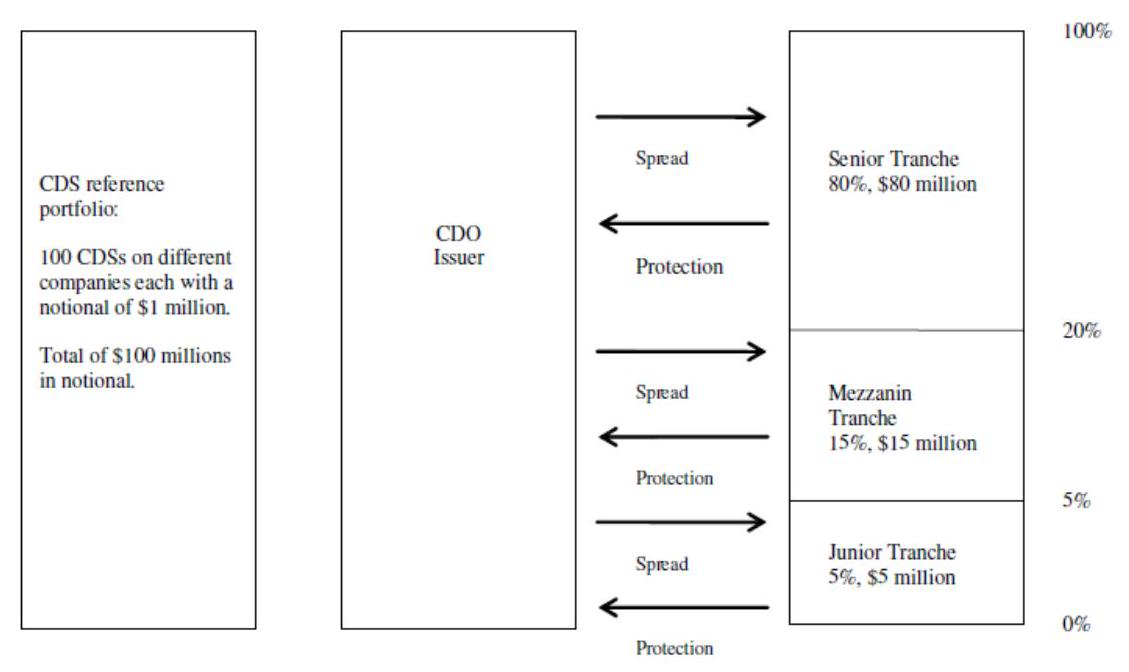
\includegraphics[width=0.8\textwidth]{figures/cdo.jpg}
\captionsetup{labelformat=empty}
\caption{Figure: Structure in an unfunded synthetic CDO.}
\end{center}
\end{figure}

with $\eta$ being grid size. Using LPA, pricing of a tranche boils down to evaluating

$$
\E\left[Z_{j, t_{k}}\right]=\int_{0}^{1} \min \left\{(1-R) \theta, K_{U_{j}}\right\}-\min \left\{(1-R) \theta, K_{L_{j}}\right\} \d  F\left(\theta ; q_{t_{k}}, \beta\right)
$$

where

$$
F\left(\theta ; q_{t_{k}}, \beta\right)=\Phi\left(-\frac{\Phi^{-1}\left(q_{t_{k}}\right)-\Phi^{-1}(\theta) \sqrt{1-\beta^{2}}}{\beta}\right) .
$$

